\documentclass[11pt, a4paper]{article}
\usepackage{blindtext}

\usepackage[utf8]{inputenc}
\usepackage[french]{babel}
\usepackage[T1]{fontenc}
\usepackage[hidelinks]{hyperref}
\usepackage{listings}
\usepackage{amsmath}
\usepackage{graphicx}
\usepackage{float}
\usepackage{dirtytalk}
\usepackage{xcolor}
\usepackage[toc,page]{appendix}
\usepackage{lstautogobble}
\usepackage[left=2cm, right=2cm, top=2cm, bottom=2cm]{geometry}
\usepackage{csquotes}
\usepackage[backend=bibtex]{biblatex}

\bibliography{references}

\renewcommand{\appendixtocname}{Annexes}
\renewcommand{\appendixpagename}{Annexes}

\definecolor{codegreen}{rgb}{0,0.6,0}
\definecolor{codegray}{rgb}{0.5,0.5,0.5}
\definecolor{codepurple}{rgb}{0.58,0,0.82}
\definecolor{backcolour}{rgb}{0.95,0.95,0.92}

\lstdefinestyle{mystyle}{
    backgroundcolor=\color{backcolour},   
    commentstyle=\color{codegreen},
    keywordstyle=\color{magenta},
    numberstyle=\tiny\color{codegray},
    stringstyle=\color{codepurple},
    basicstyle=\ttfamily\footnotesize,
    breakatwhitespace=false,         
    breaklines=true,                 
    captionpos=b,                    
    keepspaces=true,                 
    numbers=left,                    
    numbersep=5pt,                  
    showspaces=false,                
    showstringspaces=false,
    showtabs=false,                  
    tabsize=2,
    belowskip=-0.5em,
    autogobble
}

\lstset{style=mystyle}


\title{Accélération Python avec GPU\\
\large Rapport de TAL}
\author{Joseph Leonard Stephen Auguste}

\begin{document}

\maketitle
\tableofcontents

\newpage
\section{Introduction}

Ce document présente l'emploie d'\texttt{OpenCL} et du \textit{framework} 
\texttt{PyOpenCL}. Son but est de montrer comment il est possible de cibler
le GPU \textit{(Graphics Processing Unit)} pour obtenir une exécution parallèle 
avec Python dans le but d'optimiser certaines parties du code.

``\texttt{OpenCL} \textit{(Open Computing Language)} est la combinaison d’une API et d’un
langage de programmation dérivé du \texttt{C}, proposé comme un standard ouvert
par le \texttt{Khronos Group}.''\autocite{wikiopencl}. Il permet d'implémenter des 
algorithmes sur les GPU et est donc conçu pour faire du code parallèle.

Quant à \texttt{PyOpenCL}, 
c'est un \textit{framework} qui permet d'intégrer du code \textit{OpenCL} à
du \texttt{Python}. C'est un projet similaire à \texttt{PyCUDA} mais il a la 
particularité de ne pas être limité aux GPU \texttt{Nvidia}.
C'est aussi un projet 
\href{https://github.com/inducer/pyopencl}{\textit{open source}}.

On présentera donc d'abord les différentes architectures GPU existantes et \texttt{OpenCL}.
Puis on verra l'utilisation de \texttt{PyOpenCL}. Enfin, on montrera un exemple de développement 
de code \texttt{Python} et \texttt{OpenCL} pour la multiplication de matrices.

L'ensemble du code est disponible au lien suivant: \url{https://github.com/leonardSA/gpu\_python\_acceleration/}.


\newpage
\section{OpenCL}

Cette section est basée sur les informations consultées dans le livre 
\textit{OpenCL Programming Guide}\autocite{openclguide}. 

Dans les prochaines sections, il faut comprendre que \texttt{OpenCL} travaille 
avec une queue d'exécution et que l'ensemble des opérations permettant de l'appeller 
sont des événements ajoutés à cette queue.

\subsection{Introduction à l'OpenCL}

\texttt{OpenCL} est une couche d'abstraction des composants matériels. 
Il permet de s'appuyer sur des GPUs et CPUs pour exécuter des programmes dits 
\texttt{Kernels}. On s'intéresse ici au \texttt{GPGPU} 
\textit{(general-purpose computing on graphics processing units)}. Afin d'utiliser 
nos composants de manière efficace, la parallélisation est primordiale. On retrouve 
ainsi deux grands types de parallélisation:
\begin{itemize}
    \item \textbf{\textit{data parallelisation}}: s'utilise lorsqu'on cherche à traiter
        différentes parties des données avec une même opération
    \item \textbf{\textit{task parallelisation}}: s'utilise si on cherche à exécuter des 
        kernels en parallèle
\end{itemize}

\subsection{Modèle d'exécution \textit{(execution model)}}

Afin de pouvoir s'intéresser à comment mettre en oeuvre la parallélisation, il faut 
d'abord s'intéresser au modèle d'exécution d'\texttt{OpenCL}. Une application 
\texttt{OpenCL} est constituée de deux parties: un programme hôte et des kernels.

Le programme hôte permet d'interfacer avec les composants et d'ainsi y exécuter 
les kernels définis pour cette application (figure~\ref{fig:host_device_interaction}).
Afin de lancer un kernel, il faut lui passer un tuple de dimensions sur lequel il va 
``itérer'' afin d'appliquer le code aux données: on l'appelle le 
\textbf{\textit{global NDRange}} \textit{(N dimensions range)} qu'on notera $G$.
Lorsqu'un kernel est lancé par le programme hôte, $X_g$ \textbf{\textit{work items}} tel que 
${\displaystyle X_g = \prod_{i=0}^{N}G[i]}$ sont crées et exécutent chacun le même
kernel concurrement. Pour pouvoir paralléliser l'exécution du kernel il faut 
créer plusieurs \textbf{\textit{work groups}} (figure~\ref{fig:execution_model}).

\begin{figure}[h]
    \includegraphics[width=0.6\textwidth]{../../resources/host_device_relationship.png}
    \caption{Interaction entre les différents composants définis d'OpenCL}
    \label{fig:host_device_interaction}
\end{figure}

On suppose ici que $G$ est composé de deux dimensions tel que $G = (G_x, G_y)$.
Alors, à chaque \textit{work item} on associe une coordonnée unique $g = (g_x, g_y)$ tel que 
$g_x \in [0..G_x-1]$ et $g_y \in [0..G_y-1]$ dit identifiant global. 
Ceux-ci sont alors groupés dans des
\textit{work groups} qui eux peuvent s'exécuter parallèlement pour autant de 
\textbf{\textit{compute units}} (figure~\ref{fig:host_device_interaction}) existants. 
Le nombre d'éléments crées par \textit{work group} 
est défini par le \textbf{\textit{local NDRange}} qu'on notera $L = (L_x, L_y)$. 
Grâce à $L$ on obtient le \textit{NDRange} des \textit{work groups} qu'on notera $W = (W_x, W_y)$ 
tel que 
$$L_x = G_x / W_x$$ 
$$L_y = G_y / W_y$$ 
Cela a pour conséquence que $G_x \bmod W_x = 0$ et 
$G_y \bmod W_y = 0$. Cela a aussi pour conséquence que le nombre d'éléments $X_w$ dans 
un \textit{work group} est ${\displaystyle X_w = \prod_{i=0}^{N}L[i]}$ 
(figure~\ref{fig:execution_model}). 

\begin{figure}[h]
\begin{center}
    \includegraphics[width=0.9\textwidth]{../../resources/execution_model.png}
    \caption{Modèle d'exécution d'OpenCL avec le détail des \textit{work groups} 
    et \textit{work items}}
    \label{fig:execution_model}
\end{center}
\end{figure}

Ces identifiants sont importants car ils nous permettent de comprendre comment parcourir 
l'ensemble de nos éléments dans les différentes régions de la mémoire vues dans la 
prochaine sous-section.

\subsubsection{Modèle de mémoire \textit{(memory model)}}\label{sec:memory_model}

Le modèle de mémoire se base sur des \textit{memory objects}, il en existe deux types:
\begin{itemize}
    \item \textbf{\textit{buffer objects}}: block continue de données de n'importe quels types 
        (il est possible de passer des structures)
    \item \textit{image objects}: objet spécialisé pour le traitement d'images
\end{itemize}

Avant de voir les interactions hôte-composant, on doit d'abord s'intéresser aux 
5 distinctes \textbf{régions de mémoire} (Figure~\ref{fig:memory_model}):
\begin{itemize}
    \item \textbf{\textit{host memory}}: la mémoire de l'hôte disponible uniquement 
        pour celui-ci
    \item \textbf{\textit{global memory}}: la mémoire globale disponible à tous les 
        \textit{work items} en écriture et lecture
    \item \textbf{\textit{constant memory}}: la mémoire constante disponible à tous 
        les \textit{work items} uniquement en lecture
    \item \textbf{\textit{local memory}}: la mémoire locale disponible à tous les 
        \textit{work items} d'un même \textit{work group}
    \item \textbf{\textit{private memory}}: la mémoire privée disponible uniquement 
        au \textit{work item} qui la déclare
\end{itemize}

Pour avoir accès aux données de l'hôte, il nous faut soit les copier ou les mapper 
sur le composant utilisé. Ces interactions sont définies par l'hôte. On passe par 
des buffers afin de pouvoir les rendre accessible au kernel. Ces opérations peuvent 
êtres bloquantes, on s'assure alors que la donnée est prête, ou non bloquantes 
alors le programme hôte reprend dès que l'événement a été rajouté à la queue. 
Ces buffers seront accessibles depuis la mémoire globale après avoir été passés en
arguments (voir Section~\ref{sec:execution_kernel}).

\begin{figure}[h]
\begin{center}
    \includegraphics[width=0.9\textwidth]{../../resources/memory_model.png}
    \caption{Modèle de mémoire d'OpenCL}
    \label{fig:memory_model}
\end{center}
\end{figure}

\subsubsection{Le Kernel}

Le kernel s'écrit en \textit{\textbf{OpenCL C}} qui est un dérivé du C99. 
Cependant, des fonctionnalités souvent utilisées en C y ont été retirées:
\begin{itemize}
    \item la récursivité
    \item les pointeurs de fonctions
    \item l'allocation dynamique
    \item les \textit{bit fields}
\end{itemize}

Des types spéciaux y ont été rajoutés tel que \textit{float4} qui permet de 
travailler directement sur des vecteurs d'ici 4 éléments. Ces types ont été 
ajoutés afin de pouvoir exploiter du parallélisme de données.
On retrouve aussi l'ajout de fonctions de synchronisation tel que \textit{barrier}.

Des exemples de kernel sont disponibles plus loin (voir Sections~\ref{sec:pyopencl}
et~\ref{sec:matrixmultiplication}).

\subsection{Installation d'OpenCL}

L'installation d'\texttt{OpenCL} passe par deux étapes:
\begin{itemize}
    \item l'installation des \textit{headers}: c’est l’API qui est définie 
        par \texttt{Khronos Group}
    \item l'installation des \textit{runtimes}: c’est l’implémentation qui est 
        définie par le vendeur du GPU (\texttt{Nvidia}, \texttt{AMD} ou 
        \texttt{Intel})
\end{itemize}

\subsubsection{L'installation des \textit{headers} sous Linux}

Cette étape passe par une ligne de commande:
\begin{lstlisting}
   sudo apt install opencl-headers
\end{lstlisting}

\subsubsection{L'installation des \textit{runtimes} d'Intel sous Linux}

Cette étape contient deux sous parties. On va d'abord installer le 
\textit{compute runtime} qui va nous permettre d'exécuter du code 
\texttt{OpenCL} sur notre machine. Les premiers paquets à installer se trouvent 
sur le github d'\texttt{Intel} \autocite{intelgit}. Le processus d'installation 
décrit ci-dessous peut aussi être trouvé à ce lien. 
\begin{lstlisting}[language=sh]
mkdir neo
cd neo
# do not copy paste, it might not be the most recent version
wget https://github.com/intel/compute-runtime/releases/download/19.14.12751/intel-gmmlib_19.1.1_amd64.deb
wget https://github.com/intel/compute-runtime/releases/download/19.14.12751/intel-igc-core_19.11.1622_amd64.deb
wget https://github.com/intel/compute-runtime/releases/download/19.14.12751/intel-igc-opencl_19.11.1622_amd64.deb
wget https://github.com/intel/compute-runtime/releases/download/19.14.12751/intel-opencl_19.14.12751_amd64.deb
wget https://github.com/intel/compute-runtime/releases/download/19.14.12751/intel-ocloc_19.14.12751_amd64.deb
# use apt install to ensure any missing dependencies will be installed
sudo apt install ./*deb         
\end{lstlisting}
\vspace{10pt}
On va maintenant installer les libraries qui vont nous permettre de compiler 
le code. Pour cela il nous faut télécharger l'archive au niveau des 
\textit{OpenCL drivers} d'\texttt{Intel} dans la section 
\textit{``Intel CPU Runtime for OpenCL''} \autocite{inteldrivers}. 
Ensuite, on installe ces derniers avant de configurer la liaison dynamique 
de la librarie \autocite{streamhpc}. Le processus est montré ci-dessous.
\begin{lstlisting}[language=sh]
# the downloaded file might not have the same name and paths may vary
tar -xvf l_opencl_p_18.1.0.015.tgz
cd l_opencl_p_18.1.0.015/rpm
# requires alien and libnuma1 - converts everything to deb packages
alien *.rpm
# use apt install to ensure any missing dependencies will be installed
sudo apt install ./*deb
# makes directories for vendors
sudo mkdir -p /usr/lib/OpenCL/vendors/
sudo mv /opt/intel /usr/lib/OpenCL/vendors/
sudo cp /usr/lib/x86_64-linux-gnu/libOpenCL.so /usr/lib/OpenCL/vendors/intel/libOpenCL.so
# configure dynamic linking
sudo echo "/usr/lib/OpenCL/vendors/intel" > /etc/ld.so.conf.d/opencl-vendor-intel.conf
sudo ldconfig
\end{lstlisting}

\subsubsection{Test de l'installation}

Un test simple de l'installation peut se faire avec la commande \textit{clinfo} 
qui permet de lister un ensemble d'information sur les composants supportant 
\texttt{OpenCL} disponible sur la machine.


\newpage
\section{OpenCL et PyOpenCL}\label{sec:pyopencl}

Cette section est basée sur la documentation de \texttt{PyOpenCL} \autocite{pyopencl}.

\subsection{Installation de PyOpenCL}
Pour installer \texttt{PyOpenCL} sous \texttt{Linux} il suffit d'entrer dans 
le terminal la commande suivante:
\begin{lstlisting}[language=sh]
    pip3 install pyopencl  
\end{lstlisting}


\subsection{Utilisation de PyOpenCL}

\subsubsection{Les types}

Afin de pouvoir respecter les types demandés par \texttt{OpenCL}, il faut 
utliser \texttt{Numpy} qui nous permet de choisir un type et un encodage spécifique 
e.g.\ le type float d'\texttt{OpenCL} requiert un encodage sur 32 bits, ainsi 
on utilise le type \texttt{numpy.float32}.

\subsubsection{Instantiation des composants GPU}

\texttt{OpenCL} étant intrinsèquement lié au matériel, il faut commencer par choisir 
le GPU sur lequel exécuter le code et instantier son contexte et sa queue 
de commande.

\begin{lstlisting}[language=python]
    import pyopencl as cl
    import numpy as np
    # choose the first platform 
    platform = cl.get_platforms()[0]       
    # retrieve platform devices to create context
    devices = platform.get_devices()        
    # create context for platform
    context = cl.Context(devices=devices)    
    # enqueue the context to make the builded programs avaiable for execution
    queue = cl.CommandQueue(context)
    ...
\end{lstlisting}

\subsubsection{Compilation du Kernel}

Il faut commencer par définir le code source du Kernel qu'on stocke dans une 
chaîne de caratères. Ensuite on crée un objet de la classe 
\texttt{pyopencl.Program} en utilisant le contexte précédemment défini. Puis 
avec la méthode \texttt{build} on compile l'exécutable de façon a récupérer 
de programme. 
\newline
\newline
\noindent{On considère le code source du Kernel qui ne fait 
qu'incrémenter chaque élément:}
\begin{lstlisting}[language=python]
program_source = """
    kernel void inc(global float * in, global float * out) {
        int id = get_global_id(0);
        out[id] = in[id] + 1;
    }
"""
\end{lstlisting}
\vspace{10pt}

\noindent{On le compile ainsi:}
\begin{lstlisting}
    ...
    # add OpenCL source code to context (source is a string)
    program_source = cl.Program(context, source)
    # compile the kernel
    program = program_source.build()
    ...
\end{lstlisting}

\subsubsection{Définitions des buffers}

On commence par définir des tableaux qui stocke nos valeurs en faisant 
attention à l'encodage. Il en faut aussi un pour le résultat.
Ensuite, à l'aide de ces derniers, on définit des \textit{buffers} du type 
\texttt{pyopencl.Buffer}. En général, on les définira uniquement avec 
les \textit{flags} \texttt{pyopencl.mem\_flags.READ\_ONLY} ou 
\texttt{pyopencl.mem\_flags.WRITE\_ONLY} par soucis de clarité et aussi car des 
optimisations peuvent êtres faites par le compilateur.
On copie ensuite les buffers entrants sur le GPU afin de pouvoir passer les 
arguments au Kernel à l'aide de la méthode \texttt{pyopencl.enqueue\_copy}. 
Il faut noter que la copie est bloquante par défaut et qu'il faut rajouter le 
paramètre positionnel \texttt{is\_blocking=False} pour le désactiver.

\begin{lstlisting}[language=Python]
...
# instantiate a numpy.ndarray of N elements of type float32 with random values
array_in = np.random.rand(N).astype(np.float32)
# instantiate a similar numpy.ndarray but filled with zeros
array_out = np.zeros(N, dtype=float32)
# create a read only buffer using array_in
buffer_in = cl.Buffer(context, flags=cl.mem_flags.READ_ONLY,
                      size=array_in.nbytes)
# create a write only buffer using array_out
array_out = cl.Buffer(context, flags=cl.mem_flags.WRITE_ONLY,
                      size=b.nbytes)
# copy array_in content onto GPU via buffer_in
# is_blocking flag set to True by default
cl.enqueue_copy(queue, src=array_in, dest=buffer_in)    
...
\end{lstlisting}


\subsubsection{Exécution du Kernel}\label{sec:execution_kernel}

On définit alors un tuple des arguments avec nos \textit{buffers}.
Ensuite pour exécuter le Kernel, il suffit d'appeller la fonction
définie dans le code source. Cependant, plus de paramètres que le tuple sont 
à lui passer:
\begin{itemize}
    \item \textbf{queue:} la queue de commande
    \item \textbf{global memory:} le \textit{global NDRange}
    \item \textbf{local memory:} le \textit{local NDRange}
    \item \textbf{kernel arguments:} le tuple des arguments préfixé d'un 
        astérique afin de déballer ces derniers
\end{itemize}
Enfin, pour récupérer le résultat on copie le contenu du \textit{buffer} de 
sortie dans notre tableau résultat.

\begin{lstlisting}[language=python]
    ...
    # Kernel function prototype: kernel void inc(global float * in, global float * out)
    kernel_arguments = (buffer_in, buffer_out)
    # run the program
    program.inc(queue,                  
                len(array_in),          # global memory 
                None,                   # local memory
                *kernel_arguments)
    # copy array_out content off GPU and onto host via buffer_out
    cl.enqueue_copy(queue, src=buffer_out, dest=array_out)
\end{lstlisting}


\newpage
\section{Multiplications de matrices}\label{sec:matrixmultiplication}

Les programmes font une multiplication de matrice tel que:

\[
A = \begin{bmatrix} 
    a_{11} & a_{12} & \dots & a_{1n}\\
    \vdots & \ddots &  \\
    a_{m1} &        & & a_{mn} 
    \end{bmatrix}
    ,
B = \begin{bmatrix} 
    b_{11} & b_{12} & \dots & b_{1p}\\
    \vdots & \ddots &  \\
    b_{n1} &        & & b_{np} 
    \end{bmatrix}
    ,
C = \begin{bmatrix} 
    c_{11} & c_{12} & \dots & c_{1p}\\
    \vdots & \ddots &  \\
    c_{m1} &        &  & c_{mp} 
    \end{bmatrix}
    ;
    AB = C
\]

Les programmes génèrent ainsi des tableaux de une dimension de tailles 
$A_{lignes} \quad * \quad A_{colonnes}$ et $B_{lignes} \quad * \quad B_{colonnes}$
avec des nombres aléatoires pour $A$ et $B$ respectivement, 
et une taille $A_{lignes} \quad * \quad B_{colonnes}$ avec des zéros pour $C$ avant 
de réaliser la multiplication.

On s'assure aussi avant de commencer tout traitement que $A_{colonnes} = B_{lignes}$.

\subsection{Implémentation naïve}  

\subsubsection{Idée de l'implémentation}

Pour l'implémentation naïve, on s'est basé sur la formule mathématique suivante:
\[
    C_{ij} = \sum_{k=1}^{n} a_{ik}b_{kj}\quad\textrm{pour}\quad i = 1, \dots, m\quad \textrm{et}\quad j = 1,\dots,p
\]

Cette formule se traduit facilement en \texttt{OpenCL} en calculant chaque $C_{ij}$ dans un \textit{work item}. 
On obtient ainsi le kernel suivant:

\begin{lstlisting}[language=c]
__kernel void matrix_mult(__global float *a,
                          __global float* b,
                          __global float* c,
                          const unsigned int a_ncol,
                          const unsigned int b_ncol) {
    int rows = get_global_id(0);    /* iterate over rows */
    int columns = get_global_id(1); /* then iterate over columns */

    /* compute value */
    float value = 0;
    for (unsigned int i = 0 ; i < a_ncol ; i++) {
        value += a[rows * a_ncol + i] * b[i * b_ncol + columns];
    }

    c[rows * b_ncol + columns] = value;
}
\end{lstlisting}    
\vspace{20pt}

Comme on peut le remarquer, on ne passe pas de matrices en tant que tel. En effet 
comme mentionné dans la Section~\ref{sec:memory_model}, les \textit{buffers} sont 
forcément des vecteurs. On peut ici voir que l'on passe la matrice $A$ via le 
premier argument et ainsi les matrices $B$ et $C$. On doit aussi passer la taille 
des colonnes de $A$ et $B$ ici appelées $a\_ncol$ et $b\_ncol$ afin de pouvoir 
parcourir les matrices mises à plats.

En partant du principe que l'ensemble des éléments pour \texttt{OpenCL} ont été 
définis (voir Section~\ref{sec:pyopencl}) et le programme compilé dans la variable 
$program$, la mise oeuvre est réalisée de la façon suivante en \texttt{Python}:
\begin{lstlisting}[language=python]
import numpy as np
import pyopencl as cl

# a_dim is a tuple with (row, column) for A
A = np.random.rand(A_dim[0] * A_dim[1]).astype(np.float32)   
# b_dim ditto
B = np.random.rand(B_dim[0] * B_dim[1]).astype(np.float32)   
C = np.zeros(A_dim[1] * B_dim[0], dtype=np.float32)

A_buffer = cl.Buffer(context, flags=cl.mem_flags.READ_ONLY, size=A.nbytes)
B_buffer = cl.Buffer(context, flags=cl.mem_flags.READ_ONLY, size=B.nbytes)
C_buffer = cl.Buffer(context, flags=cl.mem_flags.WRITE_ONLY, size=C.nbytes)

cl.enqueue_copy(queue, src=A, dest=A_buffer)
cl.enqueue_copy(queue, src=B, dest=B_buffer)

kernel_arguments = (A_buffer, B_buffer, C_buffer, A_dim[1], B_dim[1])
# .wait() to wait for the event to finish
program.matrix_mult(queue, 
                   [A_dim[0], B_dim[1]],     # global dimensions
                   None, 
                   *kernel_arguments).wait()

cl.enqueue_copy(queue, src=C_buffer, dest=C)
\end{lstlisting}
\vspace{20pt}

Comme on peut le voir, les \textit{work items} sont crées à partir d'un 
\textit{global NDRange} de deux dimensions correspondant à celles de la 
matrice C. On peut aussi noter qu'on ne fait pas usage de la mémoire locale 
le \textit{local NDRange} étant mis à \textit{None}.

\subsubsection{Résultats}

On a fait trois genres de mesures afin de voir l'éfficacité et la fiabilité 
de l'implémentation: la copie des \textit{buffers}, le temps d'exécution et 
la précision des résultats. Pour faire ces mesures on a exécuté le programme 
pour des matrices carrées de même dimension allant de 10 à 1 500 lignes/colonnes par pas de 10. 
Tous les graphes peuvent êtres retrouvées avec une meilleure résolution en annexe.

\begin{figure}[H]
\begin{center}
    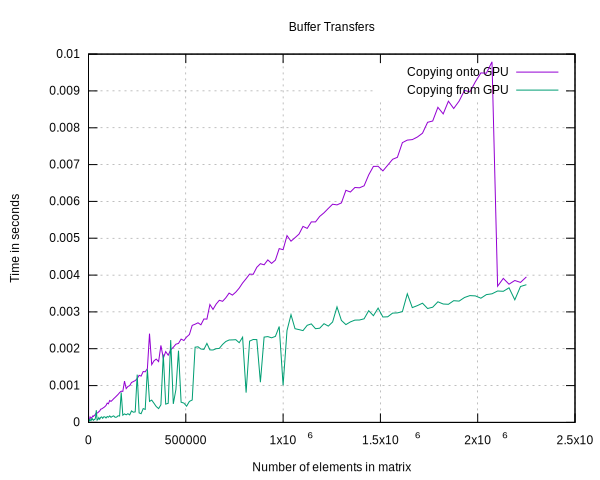
\includegraphics[width=0.6\textwidth]{../../resources/matrix_naive_buffer_transfer.png}
    \caption{Temps de copie des \textit{buffers} de \textit{float32} entre l'hôte et le GPU}
    \label{fig:buffer_transfer_naive}
\end{center}
\end{figure}

La copie des buffers est linéaire comme on peut le voir
(Figure~\ref{fig:buffer_transfer_naive}). Cependant, on constate un gain en 
temps considérable lors de la copie de \textit{A\_buffer} et \textit{B\_buffer}. 
On n'explique pas pourquoi ce gain de temps arrive à ce moment précis cependant 
on en déduit que des optimisations sont faites lorsque le nombre d'élément 
transféré devient considérable. Ici le dernier transfer vers le GPU est de 
4 500 000 éléments soit 144 000 000 bits.

\begin{figure}[H]
\begin{center}
    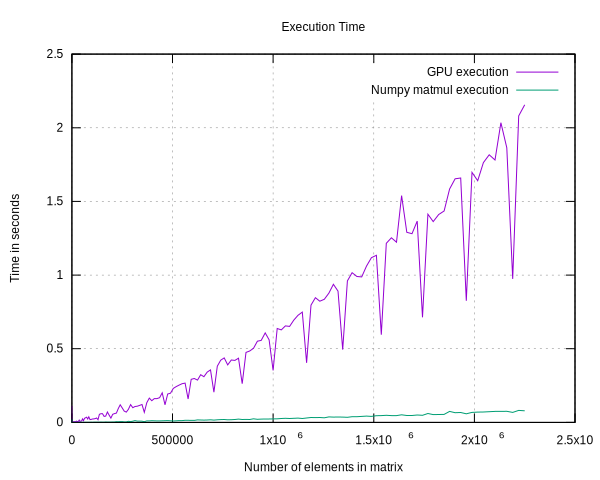
\includegraphics[width=0.6\textwidth]{../../resources/matrix_naive_execution_time.png}
    \caption{Temps d'exécution de notre implémentation et de la méthode Matmult de \texttt{Numpy}
    pour une multiplication sur des \textit{float32}}
    \label{fig:execution_time_naive}
\end{center}
\end{figure}

Le temps d'exécution de notre implémentation est comme attendu en $O(n^3)$ 
(Figure~\ref{fig:execution_time_naive}). On note cependant 
qu'elle est beaucoup plus lente que celle de \texttt{Numpy}. Cela s'explique 
par le fait que tous les \textit{work items} appertenant au même groupe, ils sont tous concurrents. 
De plus, on crée de la contention sur la mémoire global car on a autant de \textit{work items} que 
d'éléments de la matrice $C$ qui tente d'accéder concurrement à la mémoire globale. On remarque 
aussi des gains de performance réguliers qu'on n'explique pas non plus.

\begin{figure}[H]
\begin{center}
    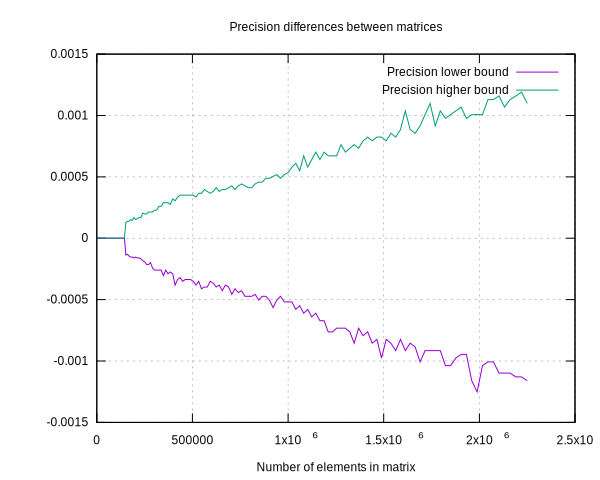
\includegraphics[width=0.6\textwidth]{../../resources/matrix_naive_float_precision.png}
    \caption{Écart de précision existant entre les résultats de la méthode Matmult de Numpy 
    et de notre implémentation pour une multiplication sur des \textit{float32}}
    \label{fig:accuracy_naive}
\end{center}
\end{figure}

Enfin, on constate un écart entre les éléments des matrices résultantes de \texttt{Numpy} et 
de notre implémentation (Figure~\ref{fig:accuracy_naive}). C'est une problématique de calcul 
sur les flottants\footnote{On ne sait pas lequel est le plus précis, la conversion en type \textit{Decimal} 
de \texttt{Python} étant très contraignante}. On peut voir sur la Figure~\ref{fig:accuracy_naive_integers} pour lequel
le calcul a été éffectué sur des entiers que nous n'avons pas d'écarts.

\begin{figure}[H]
\begin{center}
    \includegraphics[width=0.6\textwidth]{../../resources/naive_integer_accuracy.png}
    \caption{Écart de précision existant entre les résultats de la méthode Matmult de Numpy 
    et de notre implémentation pour une multiplication sur des \textit{int32}}
    \label{fig:accuracy_naive_integers}
\end{center}
\end{figure}

\subsection{Implémentation non naïve}  

\subsubsection{Idée de l'implémentation}

Cette implementation est tirée du livre \textit{OpenCL Programming Guide}\autocite{openclguide}. 
Son but est de faire usage des \textit{work groups}. Pour cela on fait des tranches de lignes 
dans la matrice afin de les passer à différents \textit{work groups} pour que chaque \textit{work item} 
calcule une ligne de la matrice $C$ (Figure~\ref{fig:non_naive_implementation_principle}). 
\begin{figure}[h]
\begin{center}
    \includegraphics[width=0.6\textwidth]{../../resources/non_naive_implementation_principle.png}
    \caption{Séparation d'une matrice en quatres \textit{work groups}}
    \label{fig:non_naive_implementation_principle}
\end{center}
\end{figure}
De plus, on s'intéresse aux types de mémoire étant donné qu'écrire 
directement dans la mémoire globale causerait des contentions et donc des pertes de performances. 
Les deux autres types de mémoire ici utilisées sont la mémoire locale et la mémoire privée: 
\begin{itemize}
    \item la mémoire locale nous sert à garder les colonnes de la matrice et elle est utilisée par l'ensemble des
        \textit{work items} d'un \textit{work group}
    \item la mémoire privée nous sert à garder les lignes de la matrice car elle n'est utilisée que par un \textit{work
        item}
\end{itemize}
On obtient ainsi le kernel suivant:
\begin{lstlisting}[language=c]
/* #define AWRK_SIZE is added by the host program */
__kernel void matrix_mult(__global float* A,
                          __global float* B,
                          __global float* C,
                          __local float* Bwrk,  /* local memory of b column for work group */
                          const int ncol) {
    int i = get_global_id(0);
    int iloc = get_local_id(0);
    int nloc = get_local_size(0);

    float Awrk[AWRK_SIZE];  /* private memory of a column for work item */

    if (i < ncol) {
        /* copy elements in private memory */
        for (int k = 0 ; k < ncol ; k++) {
            Awrk[k] = A[i * ncol + k];
        }

        for (int j = 0 ; j < ncol ; j++) {
            /* copy elements in local memory */
            for (int k = iloc ; k < ncol ; k = k + nloc) {
                Bwrk[k] = B[k * ncol + j];
            }
            barrier(CLK_LOCAL_MEM_FENCE);
            float tmp = 0.0;
            for (int k = 0 ; k < ncol ; k++) {
                tmp += Awrk[k] * Bwrk[k];
            }
            C[i * ncol + j] = tmp;
        }
    }
}
\end{lstlisting}
\vspace{20pt}

Comme on peut le voir, on passe toujours les matrices par la mémoire globale. 
On définit aussi la mémoire locale \textit{Bwrk} qui est vide au 
départ. En effet, on la remplie à chaque fois que l'on change de colonne en 
itérant sur \textit{j}. On note notamment 
l'utilisation de \textit{barrier\@(CLK\_LOCAL\_MEM\_FENCE)} qui nous permet de 
nous assurer que la mémoire globale a été remplie dans son entiereté avant 
qu'aucun \textit{work item} du \textit{work group} ne commence son calcul. 
Enfin, le remplissage de la mémoire privée se fait en itérant sur la ligne 
de la matrice concernant notre \textit{work item}.

En partant du principe que l’ensemble des éléments pour OpenCL ont été définis (voir Section 3)
et le programme compilé dans la variable program, la mise oeuvre est réalisée de la façon suivante en
Python:
\begin{lstlisting}[language=python]
import numpy as np
import pyopencl as cl

N_WORK_GROUPS = 32
# we keep size which represents a lenght of a line/colunm 
# by powers of two to be able to divide evenly everything for work groups
size = next_power_of_two32bit(max([A_dim[0], A_dim[1], B_dim[0], B_dim[1]]))    

A = np.random.rand(A_dim[0] * A_dim[1]).astype(np.float32)   
B = np.random.rand(B_dim[0] * B_dim[1]).astype(np.float32)   
C = np.zeros(A_dim[1] * B_dim[0], dtype=np.float32)

# our matrices are now of dimensions (size, size)
A = matrix_resize_with_zeros(A, size)
B = matrix_resize_with_zeros(B, size)
C = matrix_resize_with_zeros(C, size)

A_buffer = cl.Buffer(context, flags=cl.mem_flags.READ_ONLY, size=A.nbytes)
B_buffer = cl.Buffer(context, flags=cl.mem_flags.READ_ONLY, size=B.nbytes)
C_buffer = cl.Buffer(context, flags=cl.mem_flags.WRITE_ONLY, size=C.nbytes)

cl.enqueue_copy(queue, src=A, dest=A_buffer)
cl.enqueue_copy(queue, src=B, dest=B_buffer)

kernel_arguments = (A_buffer, B_buffer, C_buffer,
                    # local memory size needs to be passed for
                    # local argument
                    cl.LocalMemory(A[0].nbytes),
                    np.int32(size))
start = time.time()
program.matrix_mult(queue,
                    [size],
                    [size // N_WORK_GROUPS],
                    *kernel_arguments).wait()

cl.enqueue_copy(queue, src=C_buffer, dest=C)

matrices_resize_original_dimensions(C, A_dim[0], B_dim[1])
\end{lstlisting}
\vspace{20pt}

On remarque déjà qu'on a fait du \textit{padding} pour rendre nos matrices 
carrés. Ceci permet de nous assurer qu'il n'y aura pas de problème lors de 
la répartition des \textit{work groups}. On rappelle en effet qu'il faut que
$size \bmod N\_WORK\_GROUPS = 0$. On note aussi que l'on doit passer 
un object du type \textit{pyopencl.LocalMemory} en paramètre afin de pouvoir 
demander à \texttt{OpenCL} d'allouer tant d'octets à la mémoire locale de chaque
\textit{work group}.

\subsubsection{Résultats}

On a fait trois genres de mesures afin de voir l'éfficacité et la fiabilité 
de l'implémentation: la copie des \textit{buffers}, le temps d'exécution et 
la précision des résultats. Pour faire ces mesures on a exécuté le programme 
pour des matrices carrées de même dimension allant de 10 à 1 500 lignes/colonnes par pas de 10. 
Tous les graphes peuvent êtres retrouvées avec une meilleure résolution en annexe.
On verra que ces derniers ne sont pas concluants malgré le fait que ce soit une implémentation 
optimisée\autocite{openclguide}.


\begin{figure}[H]
\begin{center}
    \includegraphics[width=0.6\textwidth]{../../resources/buffer_transfer.png}
    \caption{Temps de copie des \textit{buffers} de \textit{float32} entre l'hôte et le GPU}
    \label{fig:buffer_transfer}
\end{center}
\end{figure}

La copie des buffers bouge par palier comme on peut le voir
(Figure~\ref{fig:buffer_transfer}). Ceci est du au \textit{padding} étant 
donné qu'un matrice de dimension (1000, 1000) par exemple sera ramené à une dimension 
de (1024, 1024). On n'explique cependant pas l'irrégularité que l'on peut observer.

\begin{figure}[H]
\begin{center}
    \includegraphics[width=0.6\textwidth]{../../resources/execution_time.png}
    \caption{Temps d'exécution de notre implémentation et de la méthode Matmult de \texttt{Numpy}
    pour une multiplication sur des \textit{float32}}
    \label{fig:execution_time}
\end{center}
\end{figure}

Le temps d'exécution de notre implémentation monte lui aussi par pallier comme attendu
(Figure~\ref{fig:execution_time}). On note cependant que notre implémentation 
est beaucoup plus lente que celle de \texttt{Numpy} et aussi que l'implémentation naïve. 
On ne l'explique pas.

\begin{figure}[H]
\begin{center}
    \includegraphics[width=0.6\textwidth]{../../resources/float_accuracy.png}
    \caption{Écart de précision existant entre les résultats de la méthode Matmult de Numpy 
    et de notre implémentation pour une multiplication sur des \textit{float32}}
    \label{fig:accuracy}
\end{center}
\end{figure}

Enfin, on constate moins d'écart entre les éléments des matrices résultantes de \texttt{Numpy} et 
de notre implémentation (Figure~\ref{fig:accuracy}). Cependant, certains pics d'écarts sont visibles. 
Ici non plus, on ne l'explique pas.

Cette partie est une incompréhension totale car cette implémentation nous est vendue comme 
une implémentation optimisée. On se demande si ce n'est pas parce qu'elle ne serait pas 
trop adapté au du matériel utilisé. Mais on l'a tout de même pris en considération, par exemple: 
l'utilisation de 32 \textit{work groups} n'est pas aléatoire, c'est parce qu'on a 32 
\textit{compute units} sur notre GPU\@. De ce fait, il aurait été intéressant de pouvoir tourner cette 
implémentation sur un autre GPU de manière à pouvoir comprendre si c'est ce dernier qui 
est à la cause de celà.


\newpage
\section{Conclusion}

\texttt{PyOpenCL} est un \textit{framework} simple d'utilisation et de prise en main 
avec une documentation officielle explicite. À l'opposé,
\texttt{OpenCL} est un language complexe. Beaucoup de notions tels que les 
modèles d'exécution et de mémoire sont à comprendre.
Même l'installation peut poser un challenge, il n'y a pas (pour \texttt{Intel}) 
de guide d'installation officiel expliquant l'ensemble des étapes. On n'a malheureusement 
pas réussi à ``le vendre'' car aucun de nos résultats n'ont été concluants. 
Cependant, il y a une raison pour laquelle \texttt{OpenCL} existe et que les
accélarations sur d'autres composants que le CPU est en essort. En imaginant qu'on 
arrive à obtenir des résultats concluants, il serait possible d'appliquer celà 
aux calculs complexes existants dans les réseaux de neurones par exemple afin 
de pouvoir accélérer l'apprentissage de l'intelligence artificielle. Dans tous 
les cas, il serait pratique pour envisager l'optimisation de \textit{bottlenecks}.
Cependant, il faut y réfléchir conséquemment avant car cela demande beaucoup 
d'investissement.


\newpage
\printbibliography{}

\newpage
\begin{appendices}
    \section{Graphes de la l'implémentation naïve de la Section~\ref{sec:matrixmultiplication}}
    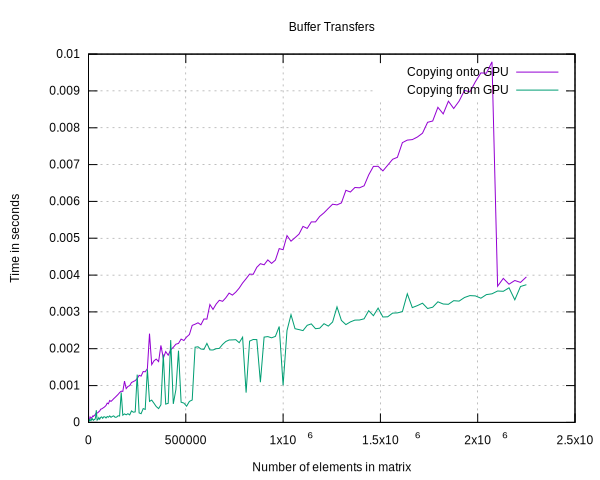
\includegraphics[width=\textwidth]{../../resources/matrix_naive_buffer_transfer.png}
    \newpage
    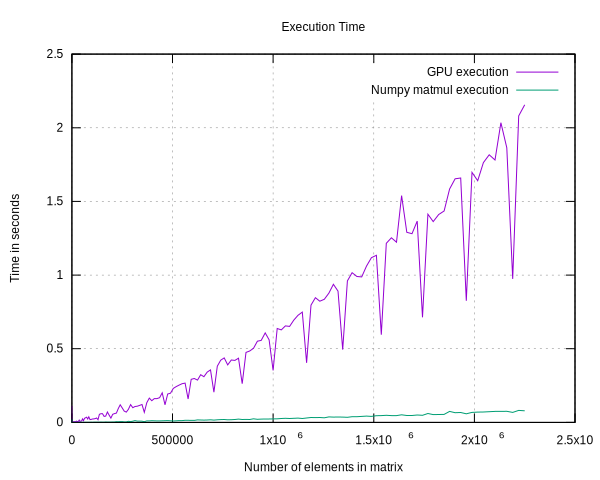
\includegraphics[width=\textwidth]{../../resources/matrix_naive_execution_time.png}
    \newpage
    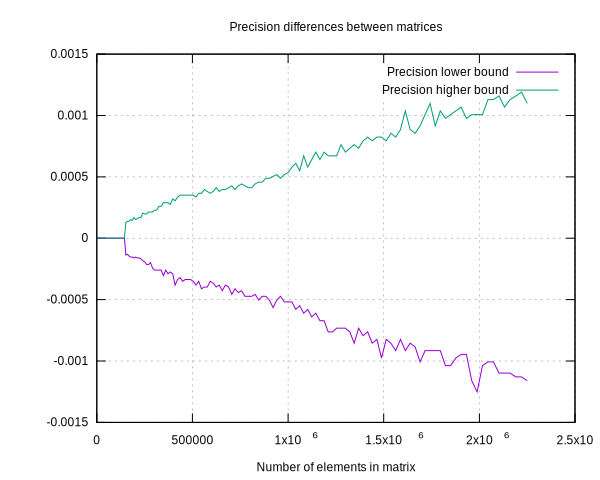
\includegraphics[width=\textwidth]{../../resources/matrix_naive_float_precision.png}
    \newpage
    \includegraphics[width=\textwidth]{../../resources/naive_integer_accuracy.png}
    \section{Graphes de la l'implémentation non naïve de la Section~\ref{sec:matrixmultiplication}}
    \includegraphics[width=\textwidth]{../../resources/buffer_transfer.png}
    \newpage
    \includegraphics[width=\textwidth]{../../resources/execution_time.png}
    \newpage
    \includegraphics[width=\textwidth]{../../resources/float_accuracy.png}
\end{appendices}

\end{document}
